\documentclass{article}
\usepackage[hmargin=1in,height=9in]{geometry}
\usepackage{algorithm,algpseudocode}
\usepackage{beton,eulervm}
\usepackage{tikz}
\usepackage{amsmath,amssymb}
\usepackage{alltt}
\usetikzlibrary{decorations.pathreplacing,shapes.multipart,matrix}
\bibliographystyle{alpha}
\begin{document}

\renewcommand{\bfdefault}{sbc}

\title{A REST Inspired Virtual File System}
\author{Louis J. Scoras \texttt{<ljsc@gwu.edu>}\\
Catalino Cuadrado \texttt{<catalino@gwu.edu>}\\
The George Washington University\\
\\
CSCI 6221 - Term Project\\
Professor Bellaachia}
\date{\today}
\maketitle

\begin{abstract}

Over the last several years, Roy Fielding's Representational State Transfer
(REST) architecture \nocite{Fie00} has had a profound impact on the design of
the web; many of the most heavily frequented webservice APIs have been
implemented using the ideas proposed by Fielding in his dissertation. Although
his paper specifically discusses REST as an implementation pattern for the
web---in particular the paper explores the intricacies of the HTTP protocol---we
believe that REST can be partially applied in other areas as well.

For our project, we will be implementing a virtual file system. We will use its
construction as a vehicle for exploring the efficacy of REST principles in
designing a generic file system. The heart of a REST service is a mapping of a
URI space to logical resources, which the client is interested in accessing.
The primary goal of a virtual file system is likewise the same. Therefore we are
confident that many of these principles can be reused. To wit, it is our
intention to leverage a framework for creating RESTful web applications as the
basis for our implementation.

As writing a file system driver from scratch would be an exhausting
process---one which might distract from the essence of our problem---we will be
making use of the FUSE project. FUSE (File System in User Space), is an API for
writing file systems which don't require kernel level access. It also provides a
greatly simplified interface for simple file systems. In addition, it has
bindings written for several high-level languages, including Ruby. Since Ruby
also hosts many successful MVC web frameworks, this makes for a natural choice.

In serving our goal of demonstrating REST as a good system for creating a file
system, we will use a readily available public web service as the provided
content of the file system. A user will be able to use normal command line and
GUI tools to browse and modify this content. As such, the main body of our
project will be dedicated to mapping HTTP verbs to their appropriate FUSE
counterparts, thereby providing the basic capabilities just described. We will
also attempt to mimic some of the more advanced parts of REST, such as resource
negotiation and caching as well.

\end{abstract}

\clearpage
\tableofcontents

\include{overview}
\section{Requirements Analysis}

\subsection{Requirements Overview}

In the following sections we will outline the project requirements. Each
requirement will have a short name, which is indicative of purpose for the
feature and is intended to for identifying the requirement. In addition, there
is a short user story, which explains the functionality in further detail.
Finally, each requirement will have a section which describes the acceptance
test which must pass for the requirement to be accepted.

The section on testing bares further discussion of terminology and notation.
Because the goal of the project is to make a file system for a POSIX
environment, it seems only right to define the desired operation in terms of
standard *NIX command line tool. Although for the project we will be creating an
automated test suite for all specified tests, it should also be possible to
verify correct operation using only tools on the command line.

As such, we will make heavy use of the following tools:

\begin{figure}[H]
\centering
\begin{tabular}{|c|c|}
\hline
COMMAND & DESCRIPTION \\\hline

ls -1 & Output each file in the directory on per line.\\

cat \textit{filename} & Output the contents of \textit{filename} to standard
output.\\

cut -d \textit{sep} -f \textit{field} & Output only the field numbered
\textit{field} using \textit{sep} to separate columns.\\

grep -i \textit{regex} & Output lines from the input that match \textit{regex}.
Case insensitive.\\

wc -l & Read the input and output the number of lines.\\

file \textit{filename} & Determine the file type of \textit{filename} and output\\\hline
\end{tabular}
\end{figure}

We assume familiarity with regular expressions and with UNIX
pipes\footnote{TODO: Add references for refreshers}. In user stories, any path
component prefixed with a ':' is to be considered a wild card, and will be
referenced by the name following the symbol.

\subsection{Static Requirements}

\newcounter{requirements}
\newenvironment{Requirements}
  {\begin{list}{SR-\arabic{requirements}.}%
               {\usecounter{requirements}}}%
  {\end{list}}

\begin{Requirements}

\subsubsection{Getting simple information}
%%%%%%%%%%%%%%%%%%%%%%%%%%%%%%%%%%%%%%%%%%%%%%%%%%%%%%%%%%%%%%%%%%%%%%%%%%%%%%%%
\item Get information for a user.

\textbf{User Story:} A user reads the file to the path \texttt{/:user/info.txt}.
Inside the file they see information regarding the user named \texttt{:user}. It
contains the following attributes:

\begin{itemize}
\item Full name
\item Screen name
\item Followers count
\item Statuses count
\item Location
\item Join date
\end{itemize}

\textbf{How to test:} The following should output "Lou Scoras".

\begin{alltt}
    \$ cat /ljsc/info.txt | grep -i 'Full-Name' | cut -d: -f2 
\end{alltt}

%%%%%%%%%%%%%%%%%%%%%%%%%%%%%%%%%%%%%%%%%%%%%%%%%%%%%%%%%%%%%%%%%%%%%%%%%%%%%%%%
\item Get a tweet given a particular id\label{req:get-a-tweet}

\textbf{User Story:} A user reads the file \texttt{/tweets/:tweet\_id.txt}.
The contents of the file will have the body of the tweet, which will contain:

\begin{itemize}
\item Message
\item Date
\item Author
\end{itemize}

If the user wants only the message contents, they can read the contents of
\texttt{/tweets/:tweet\_id/body.txt} alone.

\textbf{How to test:} Using the following command on predetermined tweet
\textit{n} yields ``This is a canned tweet.``

\begin{alltt}
    \$ cat /tweets/n/body.txt
\end{alltt}

\subsubsection{Getting lists of tweets}
%%%%%%%%%%%%%%%%%%%%%%%%%%%%%%%%%%%%%%%%%%%%%%%%%%%%%%%%%%%%%%%%%%%%%%%%%%%%%%%%
\item Get a user's latest tweets\label{req:get-latest}

\textbf{User Story:} A user lists the contents of the directory
\texttt{/:user/tweets/latest}. For each tweet in the timeline there will be a
file in the directory, \texttt{:tweet\_id.txt}. The contents of this file are as
described in SR-\ref{req:get-a-tweet}.

\textbf{How to test:} Take any tweet in a user's timeline within the last $n$
tweets, all of which are considered the latest. Let this tweets id be
\textit{tweet\_id}. The following command should then output $1$.

\begin{alltt}
    \$ ls -1 /vegasfs/tweets/latest | grep -i "\textit{tweet\_id}.txt" | wc -l
\end{alltt}

%%%%%%%%%%%%%%%%%%%%%%%%%%%%%%%%%%%%%%%%%%%%%%%%%%%%%%%%%%%%%%%%%%%%%%%%%%%%%%%%
\item Get a user's @mentions

\textbf{User Story:} This directory returns a user's mentions, up to 800 tweets (A
limitation by the API). To access the latest mentions, the user can list the
contents of \texttt{/:user/mentions} for the latest mentions for that user.
Also, they can fetch \texttt{/:user/mentions/:j-:k/} to list all the mentions
between the $j$th and $k$th mention in the timeline. Each file in these
directories will be \texttt{:tweet\_id.txt} and have the information as in
SR-\ref{req:get-a-tweet}.

\textbf{How to test:} For each file in the directory of mentions, we can ensure
that they all begin with `@` and contain \texttt{@:username}. The following
three commands should output the same value:

\begin{alltt}
    \$ cat /\textit{:user}/mentions/*.txt | wc -l
    \$ cat /\textit{:user}/mentions/*.txt | grep '^message:@' | wc -l
    \$ cat /\textit{:user}/mentions/*.txt | grep '^message:@' | grep '@\textit{:username}' | wc -l
\end{alltt}

\subsubsection{Updating tweets}
%%%%%%%%%%%%%%%%%%%%%%%%%%%%%%%%%%%%%%%%%%%%%%%%%%%%%%%%%%%%%%%%%%%%%%%%%%%%%%%%
\item Create a new tweet\label{req:create-tweet}

\textbf{User Story:} This feature allows creation of a new tweet by writing to a
file at location \texttt{/tweets/new.txt} with the contents of your tweet. The
date and author information will be appended automatically by the twitter
system.

\textbf{How to test:} Create a new tweet.

\begin{alltt}
    \$ vi /tweets/new.txt  # edit and save
\end{alltt}

The following command should contain the message entered in the previous step.

\begin{alltt}
    \$ cat \texttt{/:user/tweets/latest/}\$(ls -lt1 \texttt{/:user/tweets/latest} | head -n 1)
\end{alltt}


\subsubsection{Searching}
%%%%%%%%%%%%%%%%%%%%%%%%%%%%%%%%%%%%%%%%%%%%%%%%%%%%%%%%%%%%%%%%%%%%%%%%%%%%%%%%
\item Search for a hashtag

\textbf{User Story:} A user searches for a keyword among all tweets via the
hashtag metadata convention. When a user creates a tweet, they can prefix
keywords with the `\#` character. This search will target these tweets. The user
lists the contents of the directory \texttt{/:hashtag/tweets/}. There is one
tweet per file as described in SR-\ref{req:get-latest}.

\textbf{How to test:} Tweet a new tweet, or reuse a previous tweet for this test
as per SR-\ref{req:create-tweet}. In this tweet, create a hashtag with a GUID.
Then search for that tag as in the following command; it should output $1$.

\begin{alltt}
    \$ ls -1 /tweets/hashtag/\texttt{/\textit{GUID}/.txt | wc -l
\end{alltt}

\subsubsection{Content Negotiation}
%%%%%%%%%%%%%%%%%%%%%%%%%%%%%%%%%%%%%%%%%%%%%%%%%%%%%%%%%%%%%%%%%%%%%%%%%%%%%%%%

\item View tweets with images as images\label{req:images}

\textbf{User Story:} Users should be able to get attached media content from
tweets by changing the file extension. The if the user inspects a file
\texttt{tweet\_id.txt}, they should be able to see the picture embedded in the
tweet by opening \texttt{tweet\_id.png} for instance.

File formats that would be supported would be .png and .jpg. All embedded urls
using the yfrog service will be detected.

\textbf{How to test:} There are command-line utilities to inspect meta data
about an image file. One of these could be used to ensure that the data returned
is a valid image format. Also, we can use the UNIX \texttt{file} command to do
something similar:

\begin{alltt}
    \$ file /:user/tweets/1234.png # should return png
\end{alltt}

%%%%%%%%%%%%%%%%%%%%%%%%%%%%%%%%%%%%%%%%%%%%%%%%%%%%%%%%%%%%%%%%%%%%%%%%%%%%%%%%
\item Open a link for a given tweet as the expanded web page

\textbf{User Story:} If the embedded url is not detected as an image as in
SR-\ref{req:images}, it will be considered a normal url. If the user opens up
\texttt{tweet\_id.html}, it will return the contents of fetching that url
directly.

\textbf{How to test:} Open the file \texttt{tweet\_id.html} as described in the
story. The browser should show you the indicated page.

\end{Requirements}

\subsection{Optional Requirements}

\setcounter{requirements}{1}
\renewenvironment{Requirements}
  {\begin{list}{OR-\arabic{requirements}.}%
               {\usecounter{requirements}}}%
  {\end{list}}

\begin{Requirements}

\subsubsection{Advanced Search}
%%%%%%%%%%%%%%%%%%%%%%%%%%%%%%%%%%%%%%%%%%%%%%%%%%%%%%%%%%%%%%%%%%%%%%%%%%%%%%%%

\item Search for tweets in a geographical area

\textbf{User Story:} A user searches for nearby tweets by giving geotag
information.

The directory \texttt{/search/geo/:lat\_:long} will contain a number of files
with tweet information as in SR-\ref{req:get-latest}.

\textbf{How to test:} To test, the user would list the contents of the file
\texttt{/search/geo/xxx\_yyy/} and inspect the first file. This requirement will
be manually verified by inspecting the meta data for that tweet.

\subsubsection{Caching}

%%%%%%%%%%%%%%%%%%%%%%%%%%%%%%%%%%%%%%%%%%%%%%%%%%%%%%%%%%%%%%%%%%%%%%%%%%%%%%%%
\item Requests for tweets are cached between calls

\textbf{User Story:} A user gets information as in any of the static
requirements as above. If possible, the system should not re-fetch the entire
contents of the data if the cached version is fresh.

\textbf{How to test:} To be determined.

\end{Requirements}

\section{Design Specification}

\subsection{Purpose}

The problem we are trying to solve is how to map a RESTful API onto a POSIX
filespace. This allows users to browse the data in a familiar topography and
also utilize various command-line tools for browsing, manipulating, creating,
and deleting data. 

Our program is meant to be used by an average user who has a basic understanding
of file systems and command-line tools. Our goal is to abstract the process so
that the user does not need to know the specific RESTful API, he or she simply
needs to know simple file operations in order to interact with the program.

\subsection{Overview}

For demonstration purposes we are basing our implementation off of the Twitter
API\footnote{http://http://dev.twitter.com/doc}. The Ruby middleware uses Sinatra
for pairing methods with RESTful routes. We use the ruby implementation of the
FUSE (Fileystem in User SpacE) \footnote{https://rubyforge.org/projects/fusefs/}
to actually mimic a POSIX filesystem on the user's local environment. All data
will be fetched from the API.

The FUSE driver maps a file system call to an HTTP verb. This HTTP request is
sent to a local instance of a web service

\begin{alltt}
	\$ ls vegasfs/users/ljsc/tweets.txt
\end{alltt} 

which is then processed by a sinatra handler:
	
\begin{alltt}
	get 'vegasfs/users/ljsc/tweets.txt' do
	  #handler
	end
\end{alltt}

This handler method will perform the actual call to the twitter service and
return the data as key:value pairs: 

\begin{alltt}
	Twitter::API.tweets\_for\_user(params[:user])
\end{alltt}

All internal messaging will be done by passing JSON objects containing key:value
pairs for twitter data and strings for URIs and verbs.

When redirected to a URL, the system should attempt to fetch the URL and save
locally. In the case of a common image file type (jpg,gif,png) the system should
attempt to recognize it and save as the appropriate file type. In the event of
another type of file, the system should create a reference link to be opened by
a web browser. These operations should be done utilizing CURL and other command
line tools as appropriate.  

\subsection{Top Level Archetecture}

\begin{figure}[h]
\centering
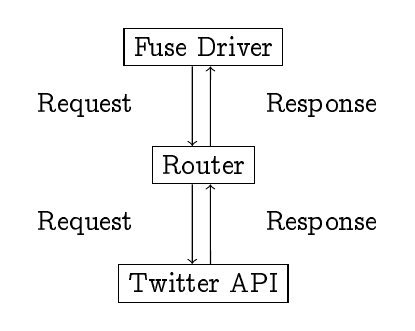
\begin{tikzpicture}
  \node [draw] at (0,3)    (Top)    {Fuse Driver};
  \node [draw] at (0,1.5)  (Middle) {Router};
  \node [draw] at (0,0)    (Bottom) {Twitter API};

  \draw [<-] (Bottom.120) -- (Middle.240);
  \draw [<-] (Middle.290) -- (Bottom.70);
  \draw [<-] (Middle.120) -- (Top.240);
  \draw [<-] (Top.290)    -- (Middle.70);

  \node at (-1.5, 0.75) { Request };
  \node at (-1.5, 2.25) { Request };
  \node at (1.5, 0.75)  { Response };
  \node at (1.5, 2.25)  { Response };
\end{tikzpicture}
\caption{Top Level Components}\label{fig:top-top}
\end{figure}

\subsubsection{Processing Elements}

\paragraph{The FUSE driver} handles file system requests generated due
to user actions on particular file paths as described in the requirements
document. It converts these requests into an HTTP request which is forwared to
the Sinatra backend.

\paragraph{The Router} implements a simple HTTP web server which listens to requests from
the FUSE driver. This will be implemented using the Sinatra framework, which
will match against a requested uri and invoke a specific handler. These handlers
will be responsible for fetching/manipulating the twitter data via the
webservice api provided by twitter.

\paragraph{Twitter API} will be leveraged to actually interact with the data as
requested by the user.  We will use an open source library for interacting with
twitter to get the required data.

\subsubsection{Connecting Elements and Data Elements}

The above processing elements are connected to form a layered architecture as
shown in figure~\ref{fig:top-top} above. All connections in the diagram
represent HTTP connections. An HTTP request using one of the specified verbs
(GET/POST/PUT/DELETE) is sent to lower level components from higher level
components. Likewise, lower level components will---based upon responses further
down the stack---return HTTP responses to the layer above.

\subsection{Detailed Description}
\subsubsection{HTTP Verb to FUSE call mapping}
The mapping will attempt to match up the HTTP verbs to FUSE function calls as defined by HTTP 1.1 and FUSE reference API. Referenced in Figure \ref{fig:httpverbs}, the HTTP verbs map naturally to the FUSE filesystem functions. Along with the verb, the fuse function will be passed the route as a parameter to perform the specified operation on the specified path.   
\begin{figure}[H]
\centering
\begin{tabular}{|c|c|}
\hline
HTTP VERB & FUSE FUNCTION CALL \\\hline

GET & read()\\

HEAD & statfs() \\

POST  & write() or create() \\

PUT & rename() \\

DELETE & unlink() \\\hline


\end{tabular}

\caption{HTTP verbs to FUSE function calls}\label{fig:httpverbs}
\end{figure}



\include{tests}
\section{User Manual}\label{sec:usermanual}

\subsection{Getting Started}
In order to use the program, please make sure you have followed all the instructions in README file located at \texttt{http://github.com/ljsc/vegas}. This will ensure that the system is installed properly.

To mount the file system, just type the following into a terminal from the \texttt{vegas} directory:
\begin{alltt}
    \$ ruby -Ilib bin/vegas mount <mountpoint directory>
\end{alltt}
\bf{Example:} to mount to the directory \texttt{tweets} the you would write:
\begin{alltt}
    \$ ruby -Ilib bin/vegas mount tweets/
\end{alltt}
Unmounting the filesystem is similarly done with 
\begin{alltt}
    \$ ruby -Ilib bin/vegas umount tweets/
\end{alltt}
This must be done each time changes are made to the source code or testing in irb. 

\subsection{Unauthenticated Operations}
Twitter has a few operations that do not require you to be logged in as a user. These methods generally aren't data-intensive. 
\subsubsection{Getting User Info}\label{userinfo}
Getting user info in the application simply involves reading the file that contains the user's twitter name, without the @ symbol.\\
\begin{alltt}
    \$ cat tweets/user/<username>.txt
\end{alltt}
\bf{Example:}
Typing: 
\begin{alltt}
    \$ cat tweets/user/agentjose1.txt
\end{alltt}
provides the following output:
\begin{alltt}
   name: Catalino
   screen_name: AgentJose1
   followers: 8
   statuses: 150
   location: 
\end{alltt}
\subsubsection{Getting A Tweet by ID}
A tweet usually has a unique identifier associated with it. The program allows you to call up a specific tweet by ID with the following syntax:
\begin{alltt}
    \$ cat tweets/tweet/<GUID>.txt
\end{alltt}
\bf{Example:} Typing:
\begin{alltt}
    \$ cat tweets/tweet/89409003758690304.txt
\end{alltt}

provides the following output:
\begin{alltt}
    Text: RT @DG_rad: Boulder is ... how you say ... Awesome.
    Author:crysb
    Date Created: Fri Jul 08 19:02:22 +0000 2011
\end{alltt}

\subsubsection{Getting a twitter image}
Built into our program is the ability to perform content negotiation via HTTP. If our program detects you would like to get an image, it will automatically download and display the image to the appropriate program. For example, typing
\begin{alltt}
    \$ cat tweets/tweet/<tweet-with-yfrogurl>.txt
\end{alltt}
will yield the text of the tweet. However, if you change the syntax to 
\begin{alltt}
    \$ open tweets/tweet/<tweet-with-yfrogurl>.<jpg|png|gif>
\end{alltt}
The system will display the image requested after filtering out the HTML and redirects. 
\subsubsection{Listing Command Top Level Types}
To list available top-level objects you can access with the system, type: 
\begin{alltt}
    \$ ls tweets/
\end{alltt}
This will produce a list of top-level objects you can access:
\begin{alltt}
    hashtag tweet user
\end{alltt}



\subsection{Authenticated Operations}\label{authenticatedoperations}
Twitter has several authenticated methods that produce much more data, in addition to providing personalized access to tweets that may be marked as private. 
Configuration in the app is achieved by editing the \texttt{configure\_authentication} method in the \texttt{VegasFS::TwitterHelpers} module in the \texttt{lib/vegasfs/router.rb} file with the correct OAuth credentials. The application will then automatically authenticate before performing any task that requires authentication.
\subsubsection{Getting Latest Tweets}\label{latesttweets}
Syntax for getting the latest 20 tweets for a user's timeline:
\begin{alltt}
    \$ cat tweets/tweet/latest.txt
\end{alltt}
\bf{example:} Typing the command yields the following response:
\begin{alltt}
    Screen Name:badbanana
    Body:My new social network is an empty pickle jar that[...]
    Screen Name:crysb
    Body:Getting everyone into position for the World Record[...]
    Screen Name:ConanOBrien
    Body:In NY. I saw "Book of Mormon," then ran into [...]
    Date:Sat Jul 09 19:37:43 +0000 2011

    Screen Name:crysb
    Body:Brazilian batala players! Been seeing them everywhere lately.
    Date:Sat Jul 09 19:17:19 +0000 2011

    <continues on for 16 more tweets...>
\end{alltt}

\subsubsection{Getting Tweets By Hashtag}\label{tweetsbyhashtags}

Hashtags are unique identifiers in Twitter indicating the tweet relates to a specifc topic. Usually these are demarcated with a '\#' symbol, such as \texttt{\#FollowFriday} or \texttt{\#ispendtoomuchtimeontwitter}. \\
In order to get tweets with hashtags, use the following syntax:
\begin{alltt}
    \$ cat hashtag/<tag>.txt
\end{alltt}
where \texttt{<tag>} is the hashtag with the pound sign removed. 

\subsection{Unsupported Impementations}
\subsubsection{new tweets}
This feature has been coded but as of project due date we were unable to figure out the correct implementation with the FUSE drivers: Writing to a file \texttt{tweets/tweet/new.txt} was supposed to post that information to Twitter, but for some reason a permissions error is preventing us from being able to write to the FUSE filesystem.
\subsubsection{Tweet Ranges}
This feature has been coded into the \texttt{VegasFS::TwitterHelpers} module but a parser was never implemented in the routes due to time constraints.



\addcontentsline{toc}{section}{References}
\bibliography{project}

\end{document}

